\begin{frame}{Learning with self-supervision: pretext tasks}

  What objective could that be?

\end{frame}


\begin{frame}{Pretext tasks: Compression}

  \begin{figure}
    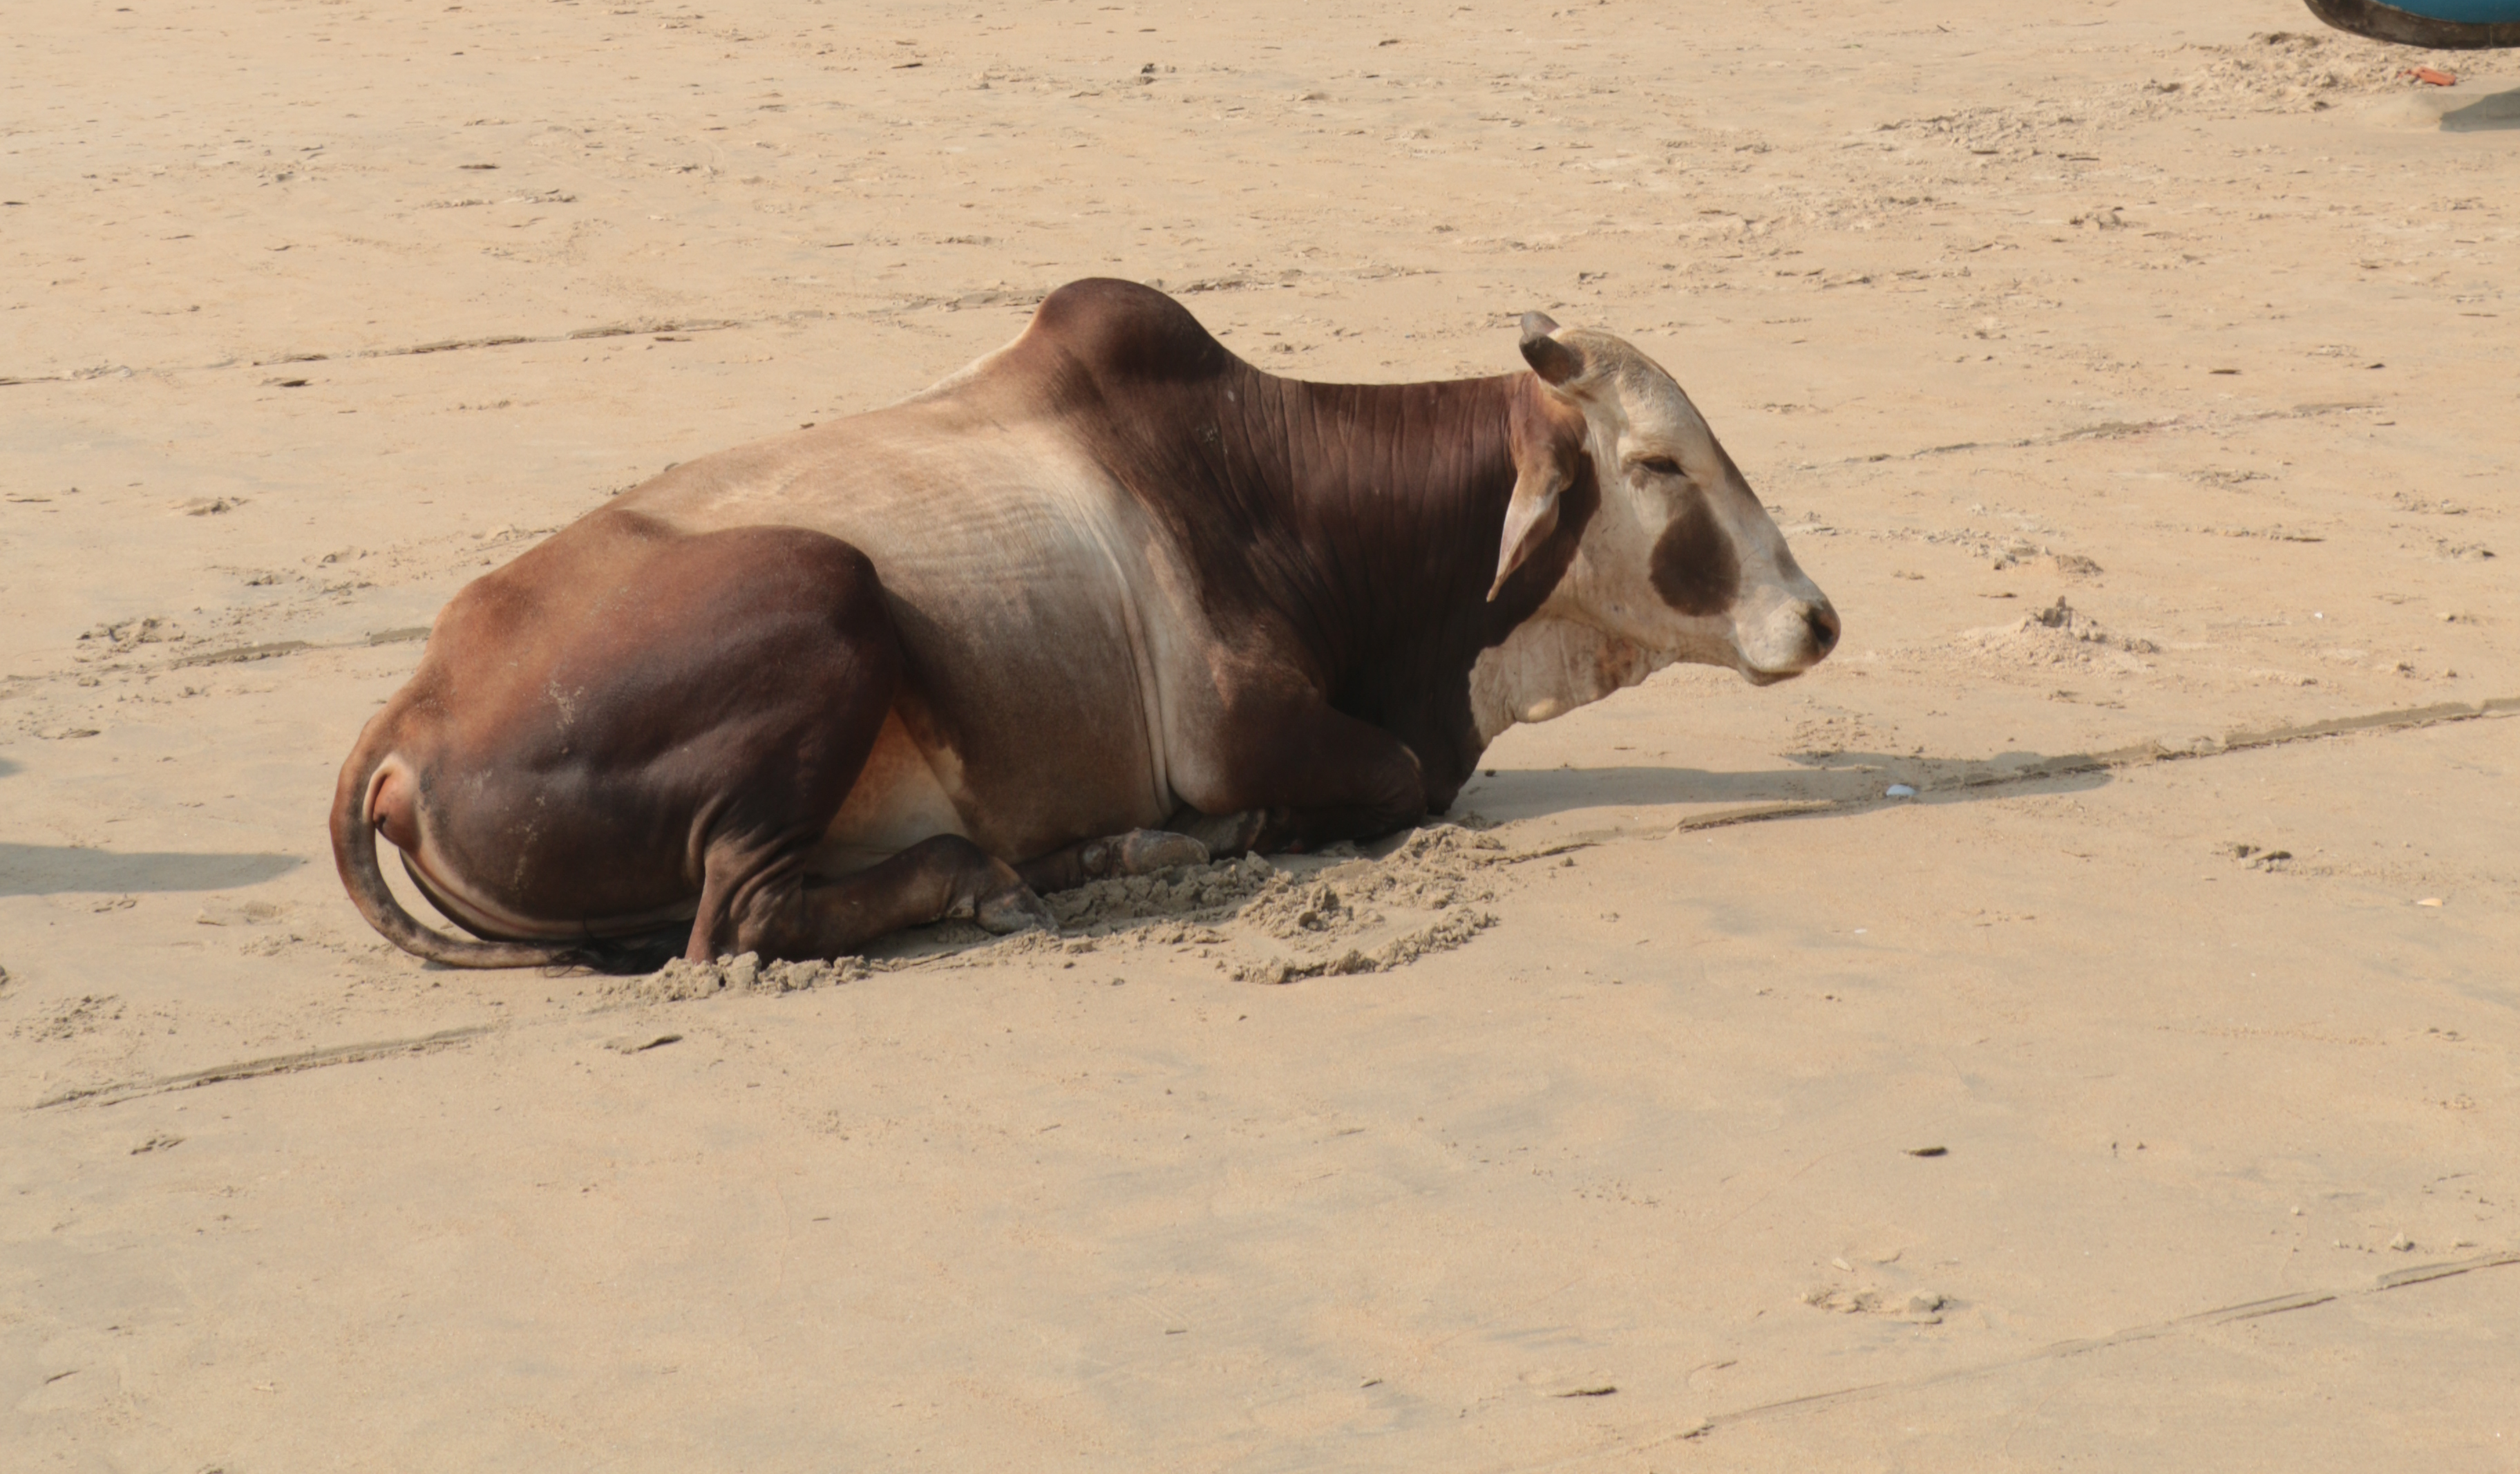
\includegraphics[width=0.24\textwidth]{cow_crop}
    \includegraphics[width=0.50\textwidth]{networks_autoencoder}
    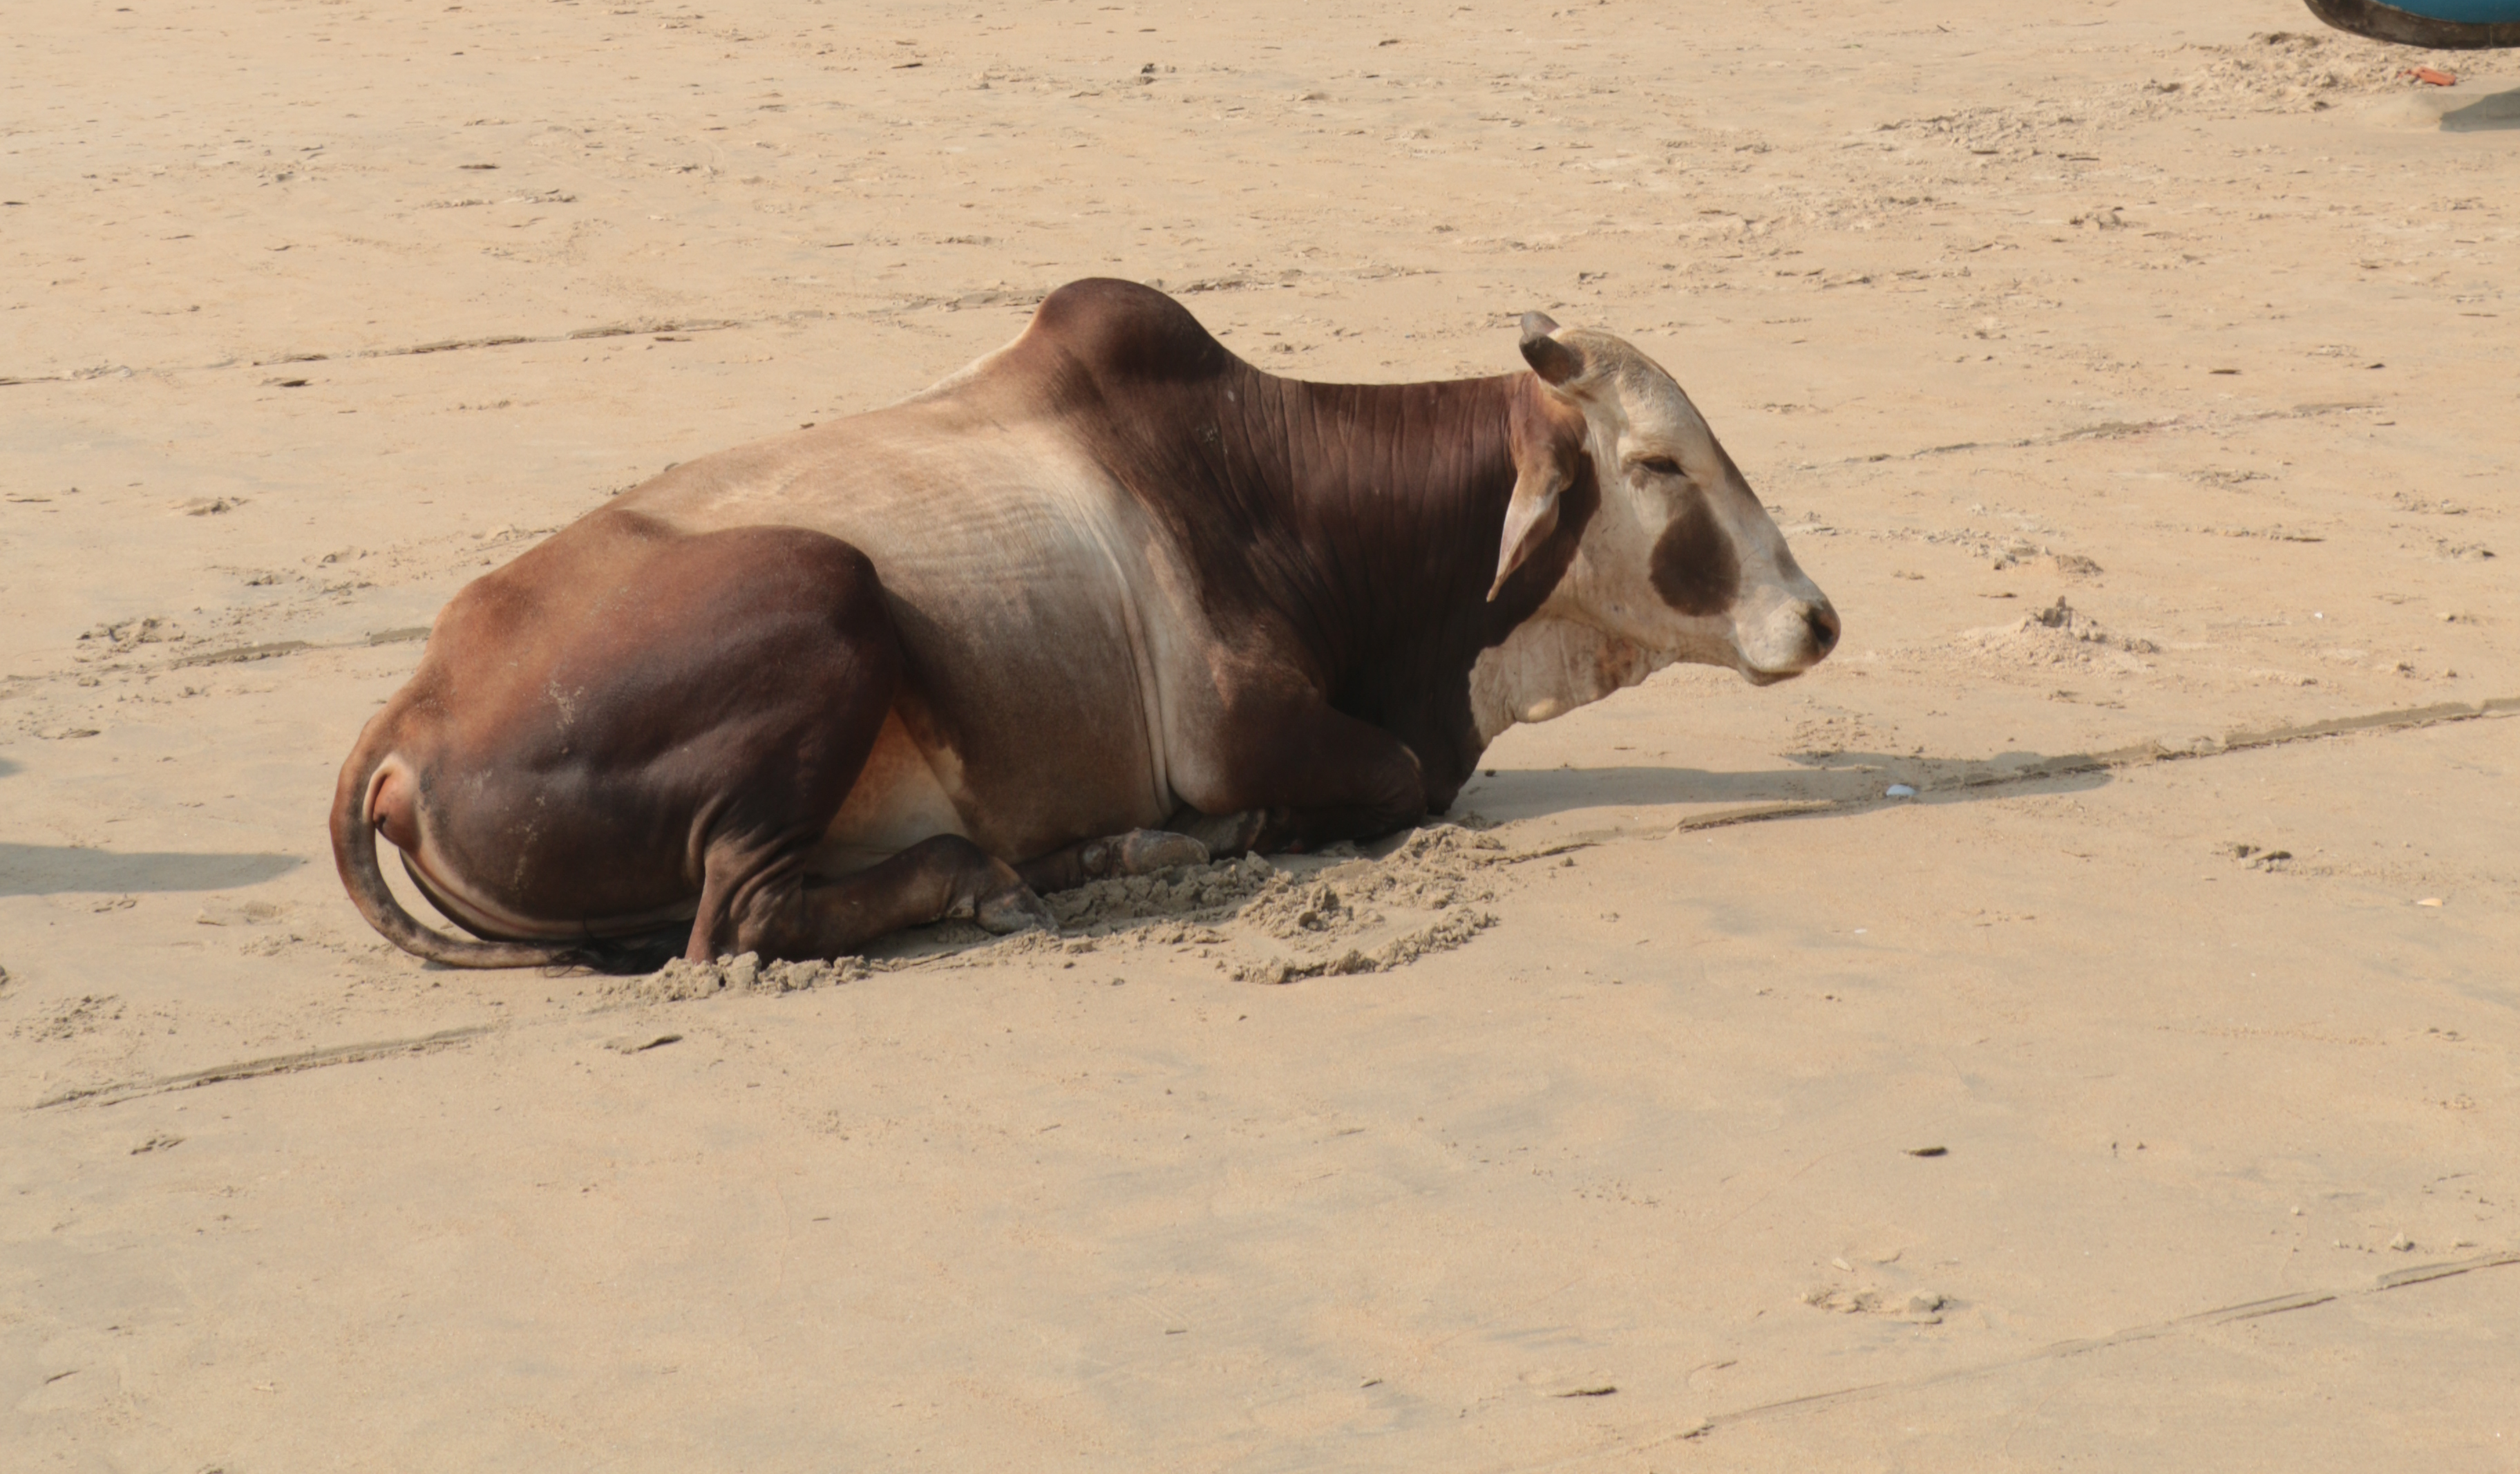
\includegraphics[width=0.24\textwidth]{cow_crop}
  \end{figure}

  \note{
    \begin{itemize}
      \item Train an autoencoding network reconstruct an image after coarse feature layer.
      \item Use encoding network for downstream task.
    \end{itemize}
  }

\end{frame}


\begin{frame}{Pretext tasks: Compression + Reconstruction}

  \begin{figure}
    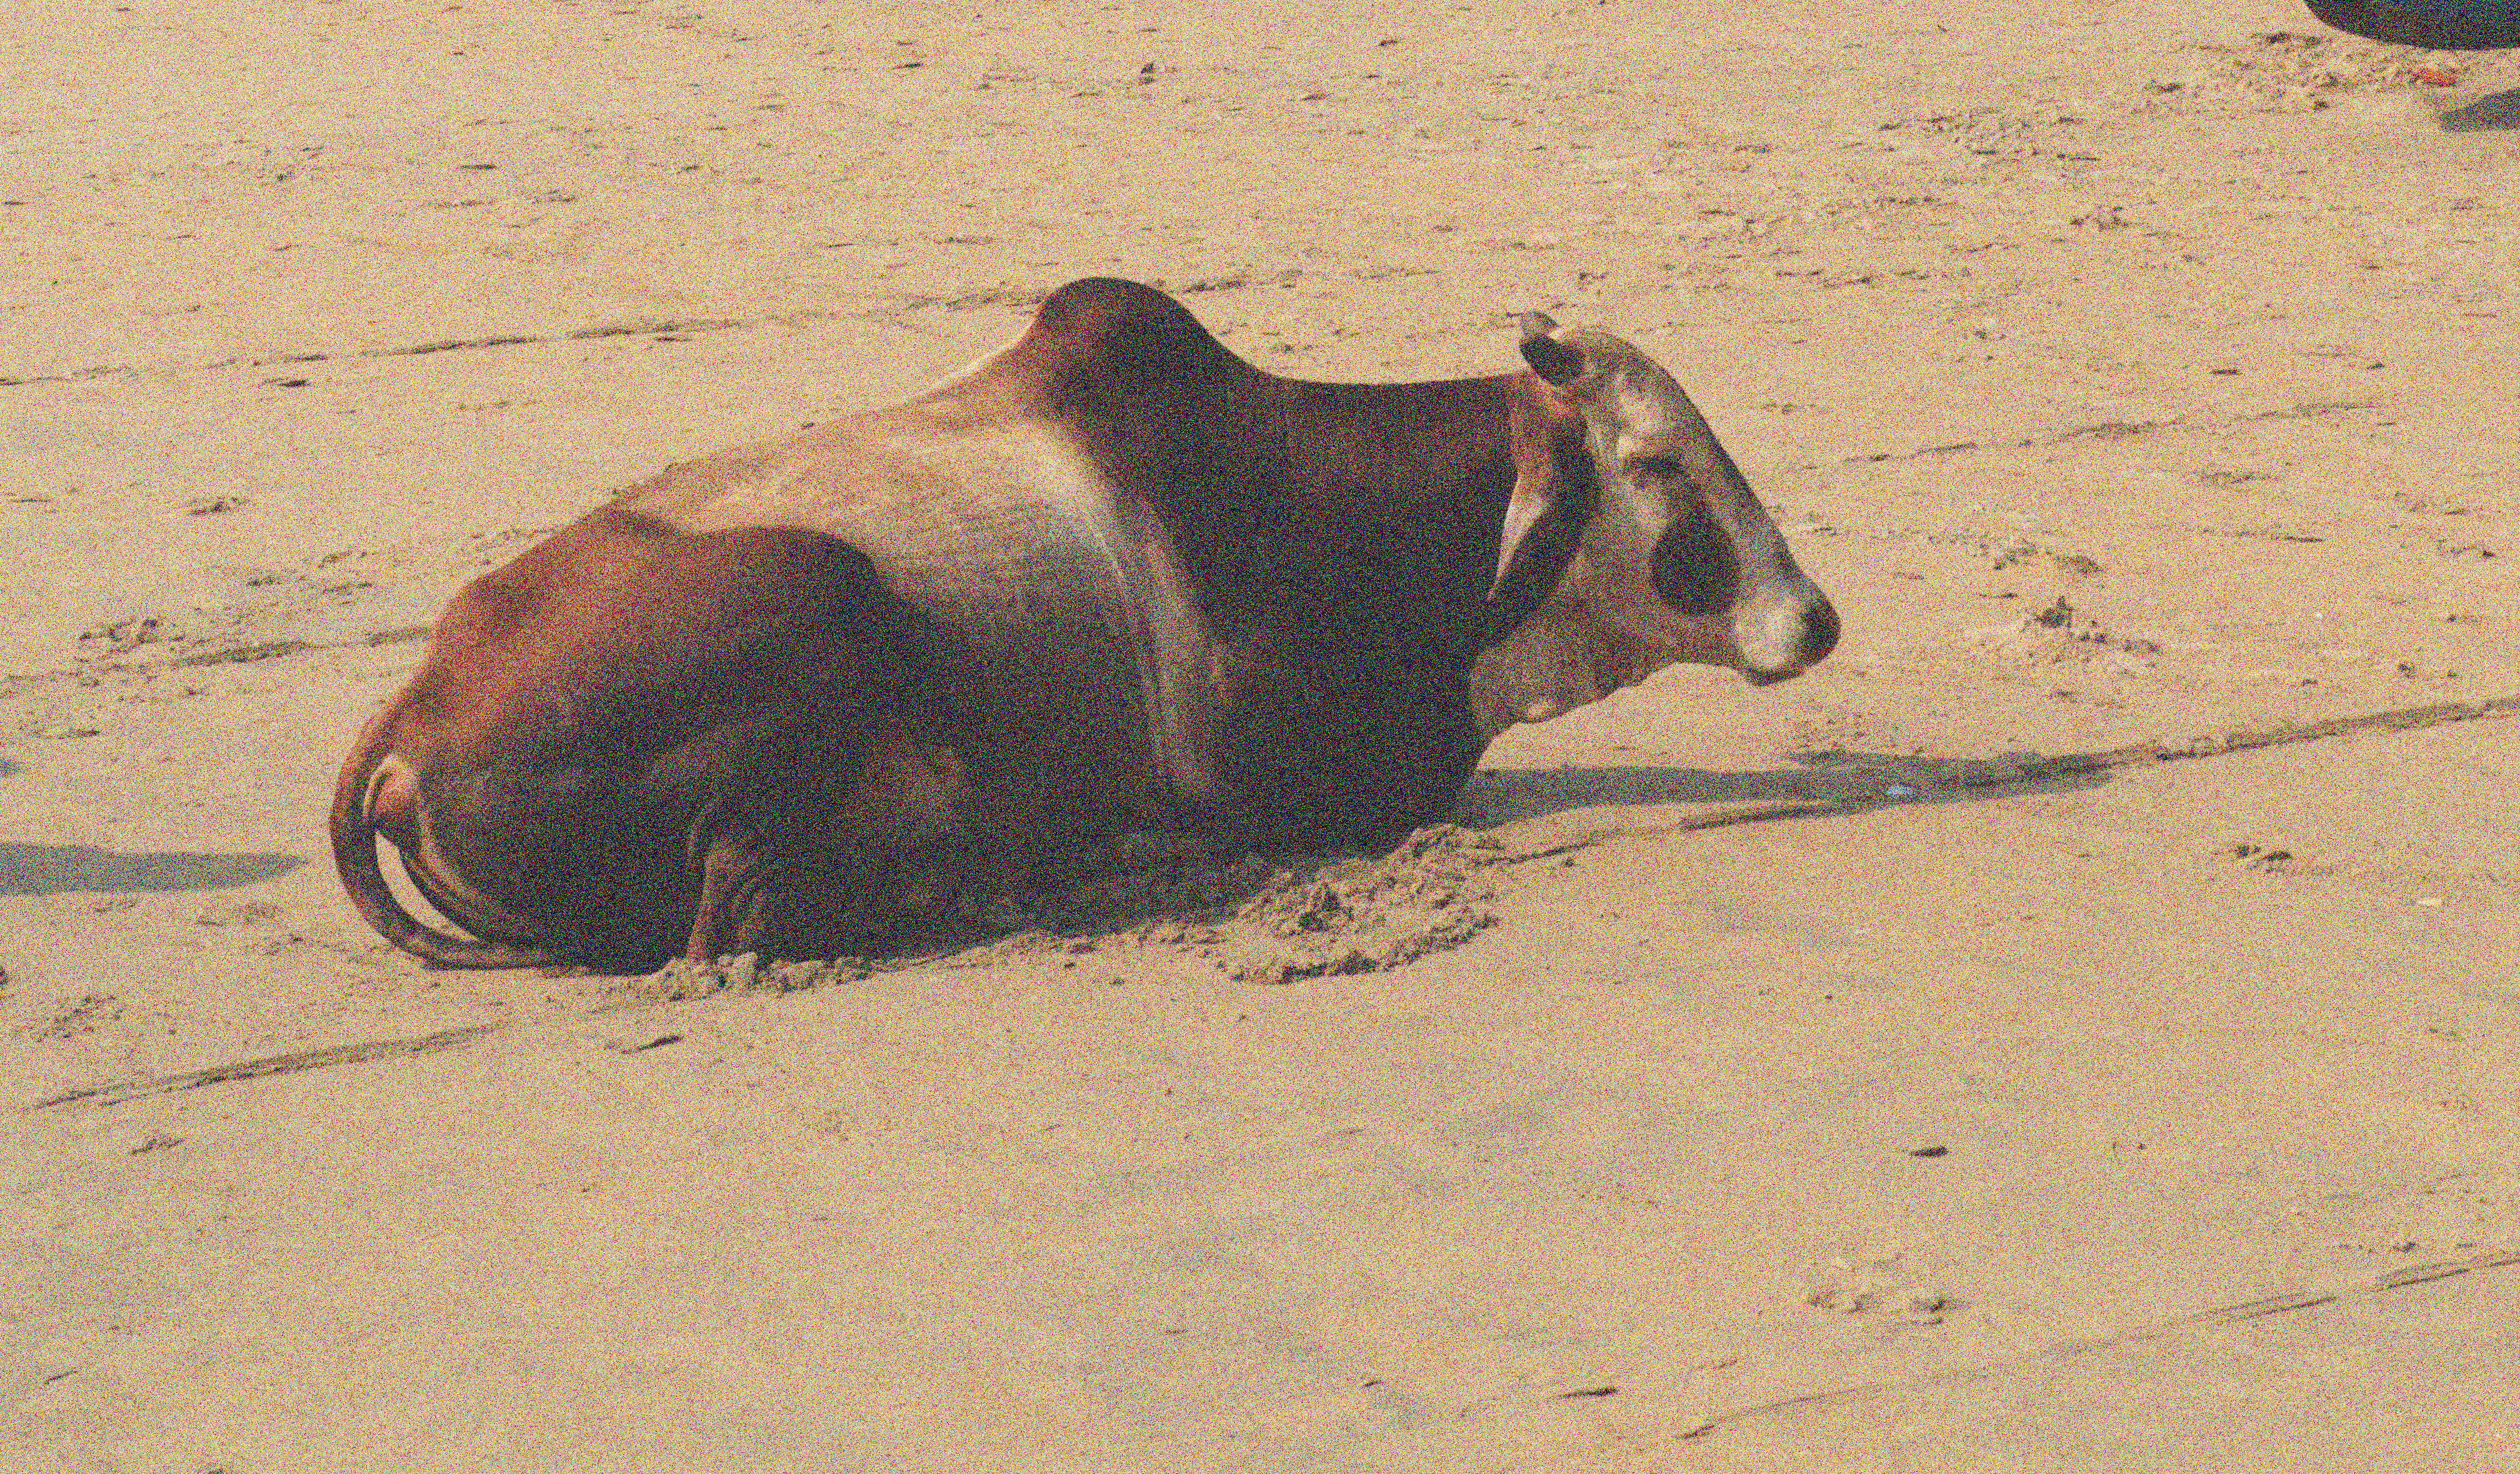
\includegraphics[width=0.24\textwidth]{cow_noise}
    \includegraphics[width=0.50\textwidth]{networks_autoencoder}
    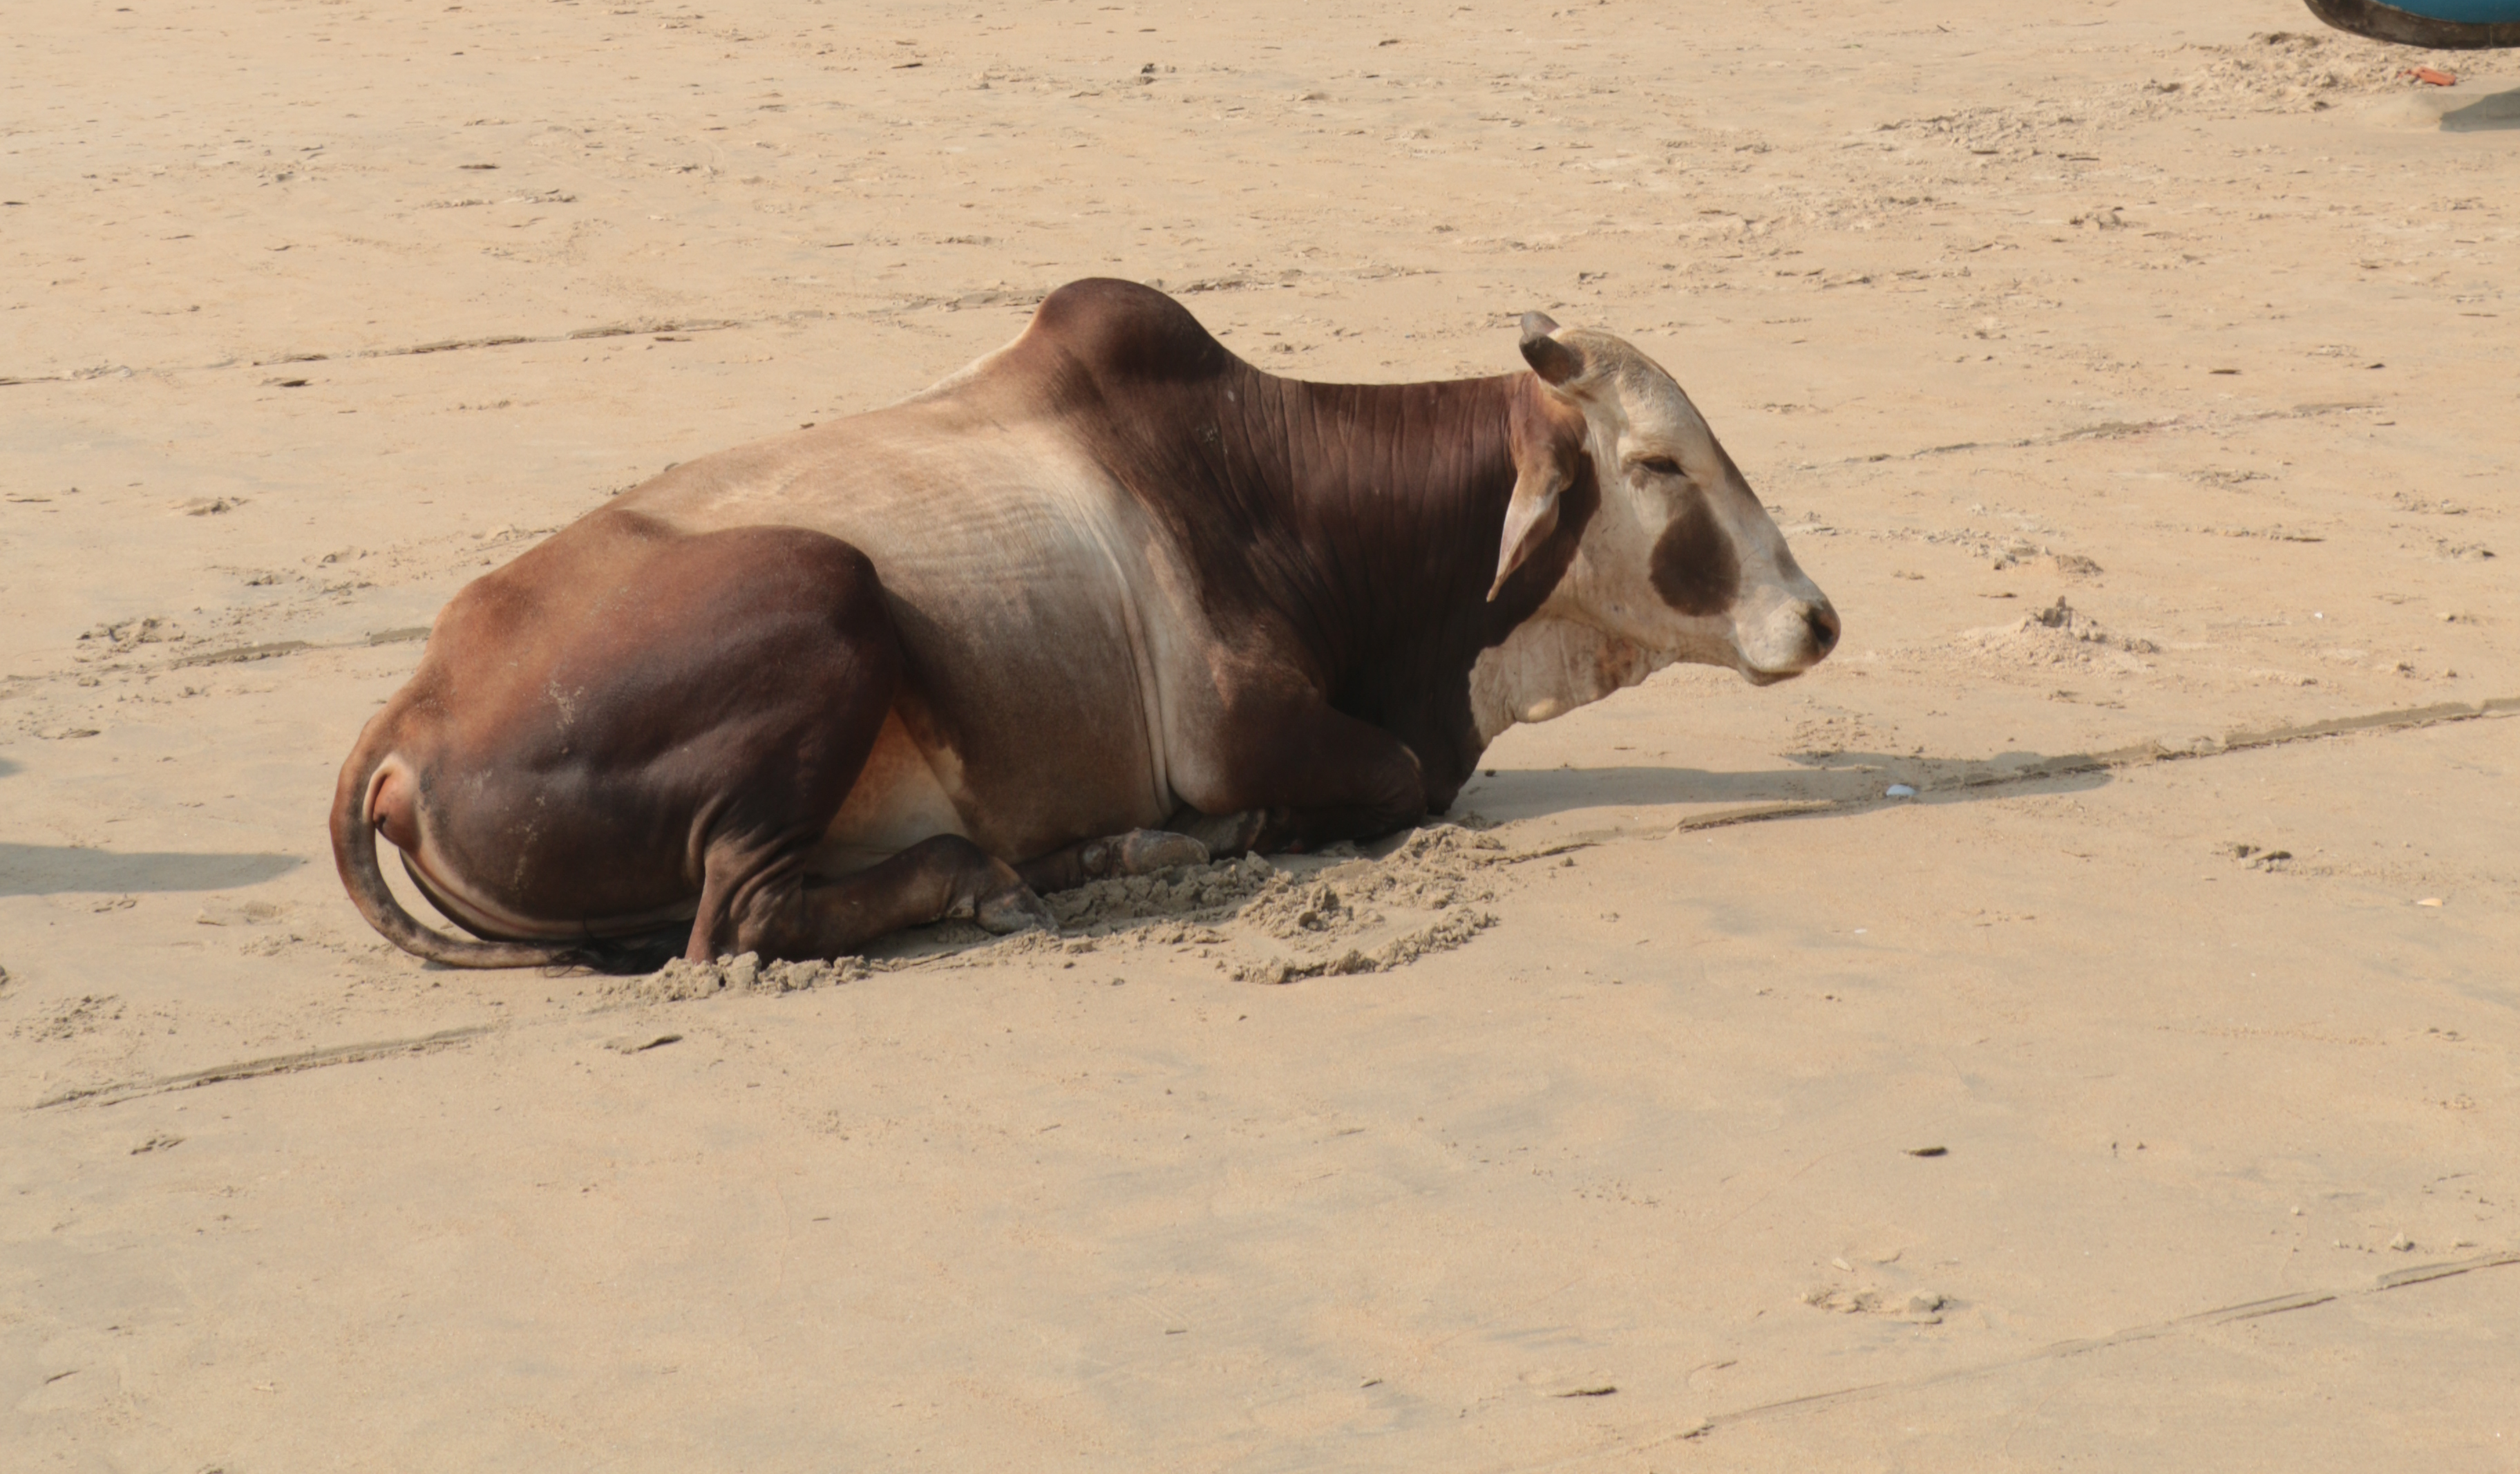
\includegraphics[width=0.24\textwidth]{cow_crop}
  \end{figure}

  \note{
    \begin{itemize}
      \item Same as before but apply distortion function $d(I)$ before feeding the image into the network.
      \item Use encoding network for downstream task.
    \end{itemize}
  }

\end{frame}


\begin{frame}{Pretext tasks: Inpainting}

  \begin{figure}
    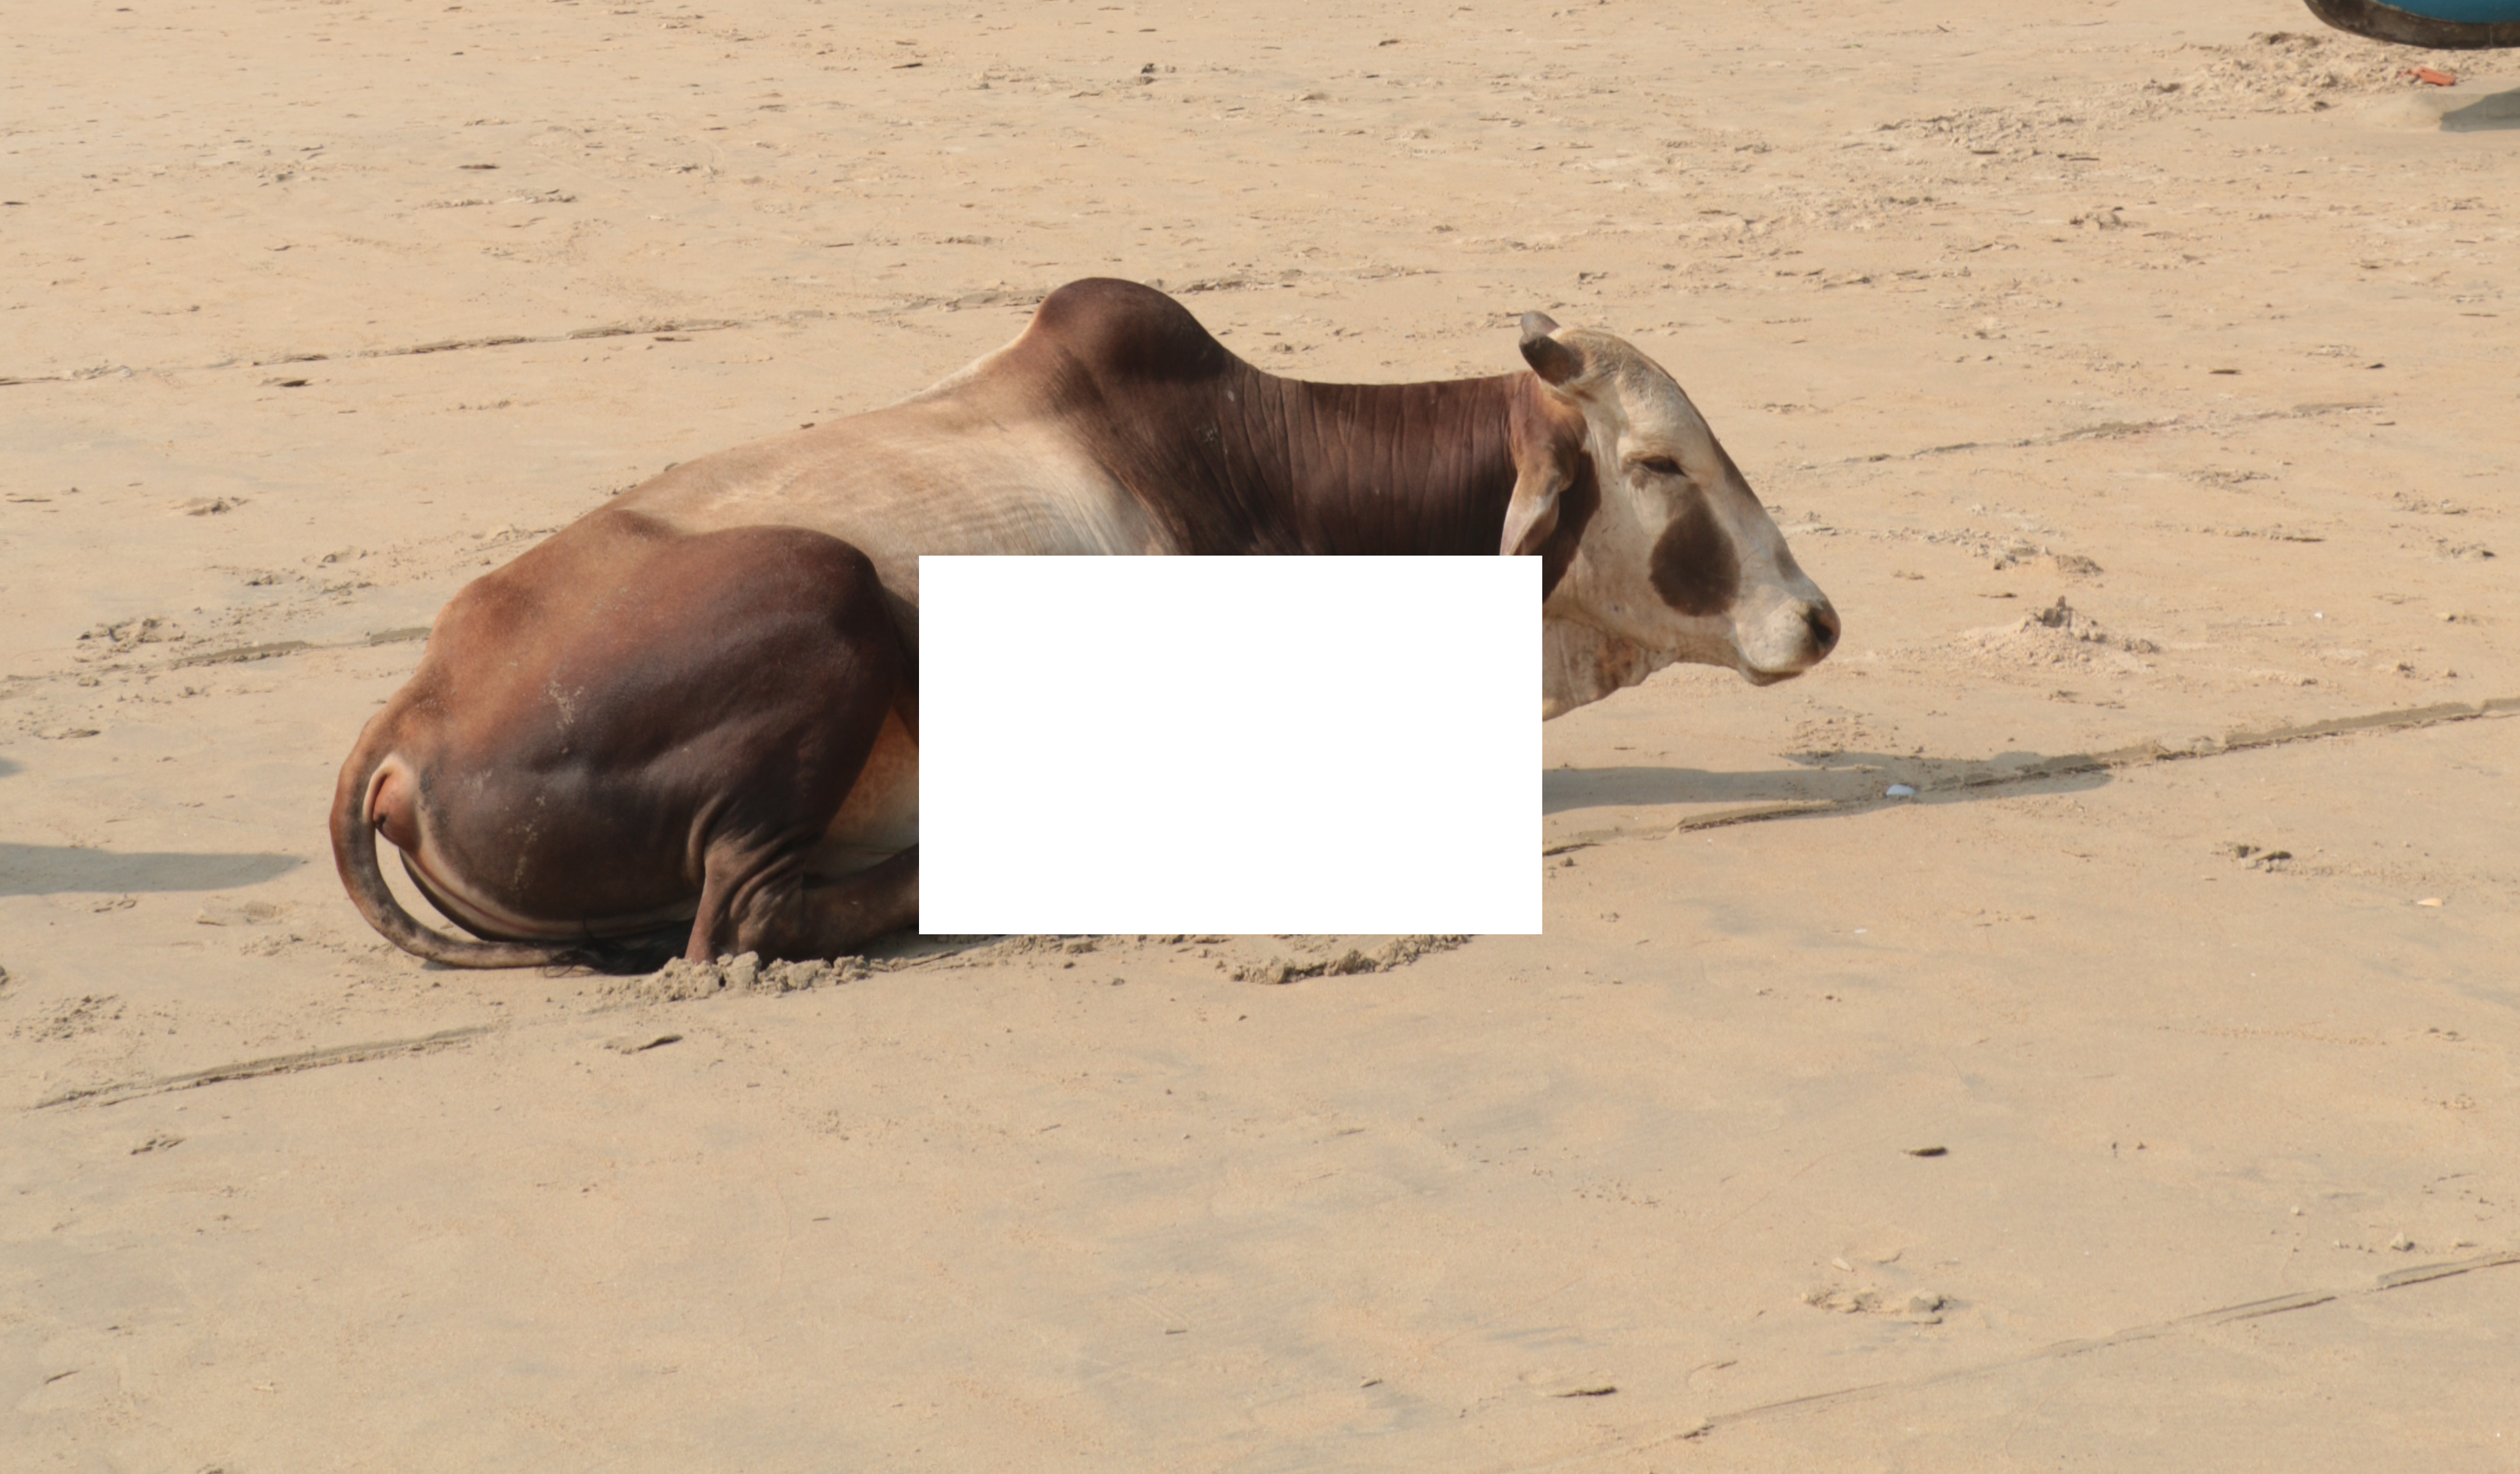
\includegraphics[width=0.24\textwidth]{cow_inpainting_00}
    \includegraphics[width=0.50\textwidth]{networks_autoencoder}
    \includegraphics[width=0.24\textwidth]{cow_inpainting_01}
  \end{figure}

  \note{
    \begin{itemize}
      \item Predict one part of the data from another.
      \item Can also be a random part of the image or e.g. the bottom half or frames of a video sequence.
      \item Context Encoders: Feature Learning by Inpainting, Pathak et al., CVPR 2016
    \end{itemize}
  }

\end{frame}


\begin{frame}{Pretext tasks: Colorization}

  \begin{figure}
    \includegraphics[width=0.24\textwidth]{cow_crop_grey}
    \includegraphics[width=0.50\textwidth]{networks_autoencoder}
    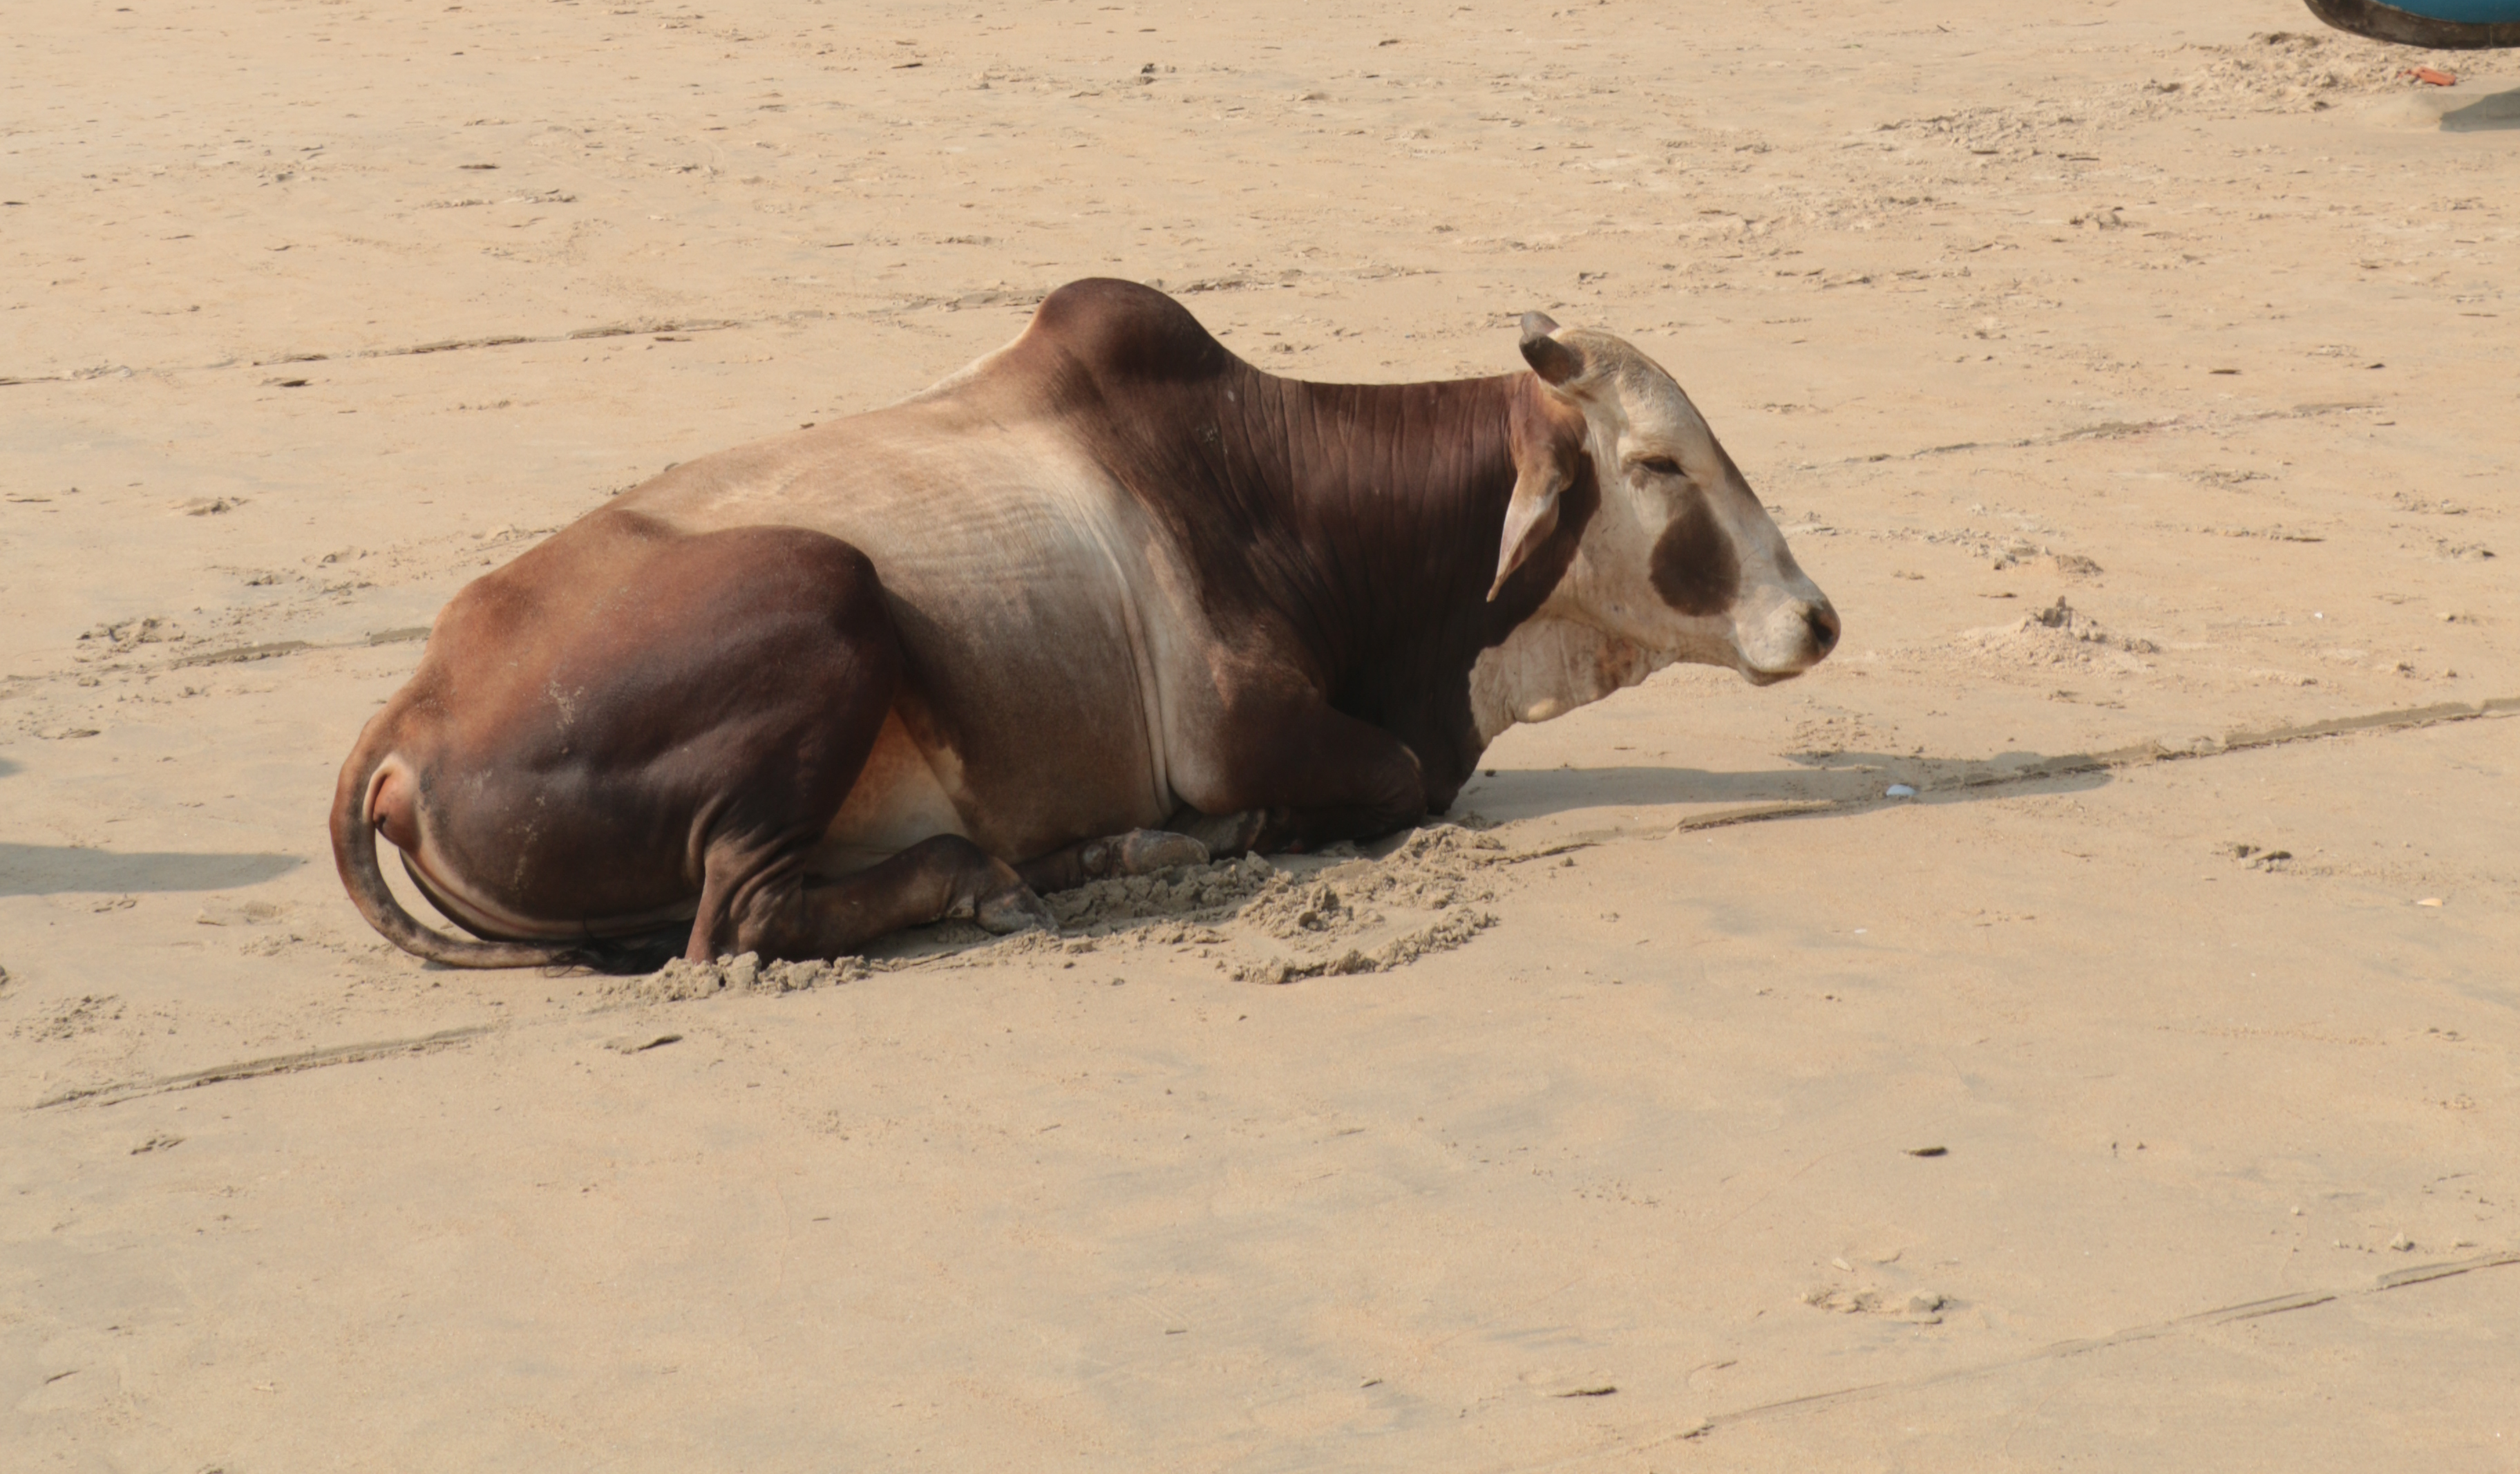
\includegraphics[width=0.24\textwidth]{cow_crop}
  \end{figure}

  \note{
    \begin{itemize}
      \item Similar to inpainting we predict a left-out property the data.
      \item Colorful Image Colorization, Zhang et al., ECCV 2016
      \item Tracking Emerges by Colorizing Videos, Vondrick et al., ECCV 2018
    \end{itemize}
  }

\end{frame}


\begin{frame}{Pretext tasks: Frame permutation}

  \begin{columns}
    \begin{column}{0.33\textwidth}
      \begin{figure}
        \includegraphics[width=0.45\textwidth]{cow_crop-0-1}\hspace{0.2mm}\includegraphics[width=0.45\textwidth]{cow_crop-1-0}\\%
        \includegraphics[width=0.45\textwidth]{cow_crop-1-1}\hspace{0.2mm}\includegraphics[width=0.45\textwidth]{cow_crop-0-0}
      \end{figure}
    \end{column}
    \begin{column}{0.43\textwidth}
      \begin{figure}
        \includegraphics[width=0.99\textwidth]{networks_encoder}
      \end{figure}
    \end{column}
    \begin{column}{0.23\textwidth}
      \begin{align*}
        {4, 2, 1, 3}
      \end{align*}
    \end{column}
  \end{columns}

  \note{
    \begin{itemize}
      \item We can also formulate the pretext task as classification problem. Here one of $n!$ possible permutations.
      \item Can also be done with video frames.
      \item Unsupervised Learning of Visual Representations by Solving Jigsaw Puzzles, Noroozi \& Favaro, ECCV 2016
    \end{itemize}
  }


\end{frame}


\begin{frame}{Pretext tasks: Frame relation}

    \begin{columns}
    \begin{column}{0.33\textwidth}
      \begin{figure}
        \includegraphics[width=0.45\textwidth]{cow_crop-0-1}\hspace{0.2mm}\includegraphics[width=0.45\textwidth]{cow_crop-1-0}\\%
      \end{figure}
    \end{column}
    \begin{column}{0.43\textwidth}
      \begin{figure}
        \includegraphics[width=0.99\textwidth]{networks_encoder}
      \end{figure}
    \end{column}
    \begin{column}{0.23\textwidth}
      \begin{align*}
        top-right
      \end{align*}
    \end{column}
  \end{columns}

  \note{
    \begin{itemize}
      \item Or as a discrete spatial relation
      \item Unsupervised Visual Representation Learning by Context Prediction, Doersch et al., ICCV 2015
    \end{itemize}
  }

\end{frame}


\begin{frame}{Pretext tasks: Transfer knowledge}

  \begin{figure}
    \includegraphics[height=0.9\textheight]{tl_00}
  \end{figure}

  \note{
    \begin{itemize}
      \item Same as for transfer learning with supervised pretraining.
      \item Replace some layers, fine tune some layers.
    \end{itemize}
  }

\end{frame}


\begin{frame}{Pretext tasks: Transfer knowledge}
  \begin{figure}
    \includegraphics[width=0.85\textwidth]{pretext_performance}
  \end{figure}
  \note{
    \begin{itemize}
      \item Problem: learned representations are very task specific
    \end{itemize}
  }
\end{frame}
